\subsubsection{22.12.15}
	Today we descussed improvements in robot that we should make.\newline
	Problems and solutions for each module:
	\begin{enumerate}
		\item Wheel base:
		\begin{table}[H]
			\vspace{-2mm}
			\begin{center}
				\begin{tabular}{|p{0.15\linewidth}|p{0.4\linewidth}|p{0.55\linewidth}}
					\hline
					Problem & Solution\\
					\hline
					Can't climb to mountain  & To try soft wheels or make mechanism that hook churro when we reach it \\	
					\hline
					Chain come off & To fix displacements of gears\\
					\hline
				\end{tabular}
			\end{center}
		\end{table}
		\item Lift and bucket:
		\begin{table}[H]
			\vspace{-2mm}
			\begin{center}
				\begin{tabular}{|p{0.15\linewidth}|p{0.4\linewidth}|p{0.55\linewidth}}
					\hline
					Problem & Solution\\
					\hline
					Bucket can't reach boxes to side  & To test and think about solution   \\	
					\hline
					Lift can't reach high box from low zone & To make mechanism that extend moving beam of the lift\\
					\hline
					The bottom of bucket is frayed & To make spare bottom part\\
					\hline
				\end{tabular}
			\end{center}
		\end{table}
		\item Gripper for debris
		\begin{table}[H]
			\vspace{-2mm}
			\begin{center}
				\begin{tabular}{|p{0.15\linewidth}|p{0.4\linewidth}|p{0.55\linewidth}}
					\hline
					Problem & Solution\\
					\hline
					Brush is too rigidly  & To install more soft tubes \\	
					\hline
					The axis is too close to bucket and prevent it's moving  & Move it forward \\	
					\hline
					When it rotates the robot shakes & To install in front part of robot beam that bond two beams where fixed wheels \\	
					\hline
				\end{tabular}
			\end{center}
		\end{table}
		
		\item Mechanism for scoring climbers - no problems.
		\item Programme of autonomous period
		\begin{table}[H]
			\vspace{-2mm}
			\begin{center}
				\begin{tabular}{|p{0.15\linewidth}|p{0.4\linewidth}|p{0.55\linewidth}}
					\hline
					Problem & Solution\\
					\hline
					There is no pushing button  & Do it  \\	
					\hline
					Robot move not accurate & Make turnings by compass and move by white line when we ride to shelter  \\	
					\hline
				\end{tabular}
			\end{center}
		\end{table}
	\end{enumerate}
\begin{itemize}
	\subsubsection{23.12.15}
		\item It was tested mechanism for turning bucket to side. It was found that it can't reach box. It was decided to change a cover so that cubes slide on it to the box.
	
		\item It was invented mechanism of extracting lift (hereinafter it will call MEL) with construction profile.
	
		\item Also today we met with other FTC team from St-Petersburg. They came to our robotics laboratory, tested their robot on our field. In addition we descussed some technical solutions and we gave them an advice how improve their robot.
	\subsubsection{26.12.15}
		\item It was came up with mount for construction profile to Tetrix beam.
		
		\item It was made the test sample MEL with construction profile.
	\subsubsection{04.01.15}
		\item The compass sensor was installed to robot. It was made turning by compass.
		
		\item We found that we can't make MEL with construction profile and decided make lift with retracktable slats.
	\subsubsection{05.01.15}
		\item It was wrote programme for moving by line.
		
		\item It was made gripper with less rigidly tubes.
		
		\item It was made programme of autonomous period for scoring climbers with using compass and light sensor. It worled stable (we tested 5 times and it worked in all cases).
		
	\subsubsection{06.01.15}
		\item It was removed lift and controllers.
		
		\item It was wrote programme for pushing button. Since the controllers of robot were removed it was tested and debuged on the Lego robot. So an algorithm is ready and we'll need to debug it on the FTC robot.
		
		\item It was made and installed on the robot tested sample of the lift with retracktable slats.
		
		\item It was decided to install controllers on the list of plywood that fixed on the side of the robot.
			
		\begin{figure}[H]
			\begin{minipage}[h]{1\linewidth}
				\center{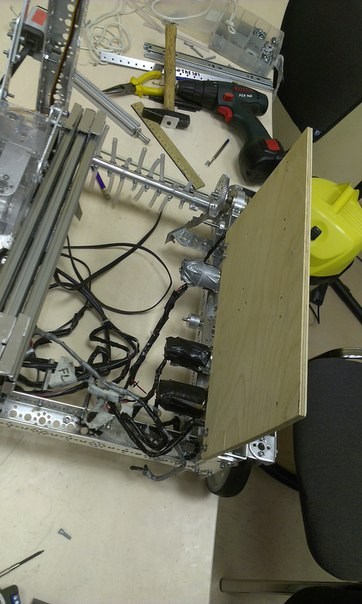
\includegraphics[scale=0.5]{days_L/Meetings/images/11}}
				\caption{Lift and new mount for controllers}
			\end{minipage}
		\end{figure}	
	\subsubsection{10.01.15}
		\item Today there was discussing of results of the last week.
		\begin{enumerate}
			\item Wheel base:
			\begin{table}[H]
				\vspace{-2mm}
				\begin{center}
					\begin{tabular}{|p{0.15\linewidth}|p{0.1\linewidth}|p{0.55\linewidth}}
						\hline
						Problem & Solution\\
						\hline
						Can't climb to mountain  &  To make mechanism that hook churro (because we didn't found other wheels that we can use)\\	
						\hline
					\end{tabular}
				\end{center}
			\end{table}
			\item Lift and bucket:
			\begin{table}[H]
				\vspace{-2mm}
				\begin{center}
					\begin{tabular}{|p{0.15\linewidth}|p{0.4\linewidth}|p{0.55\linewidth}}
						\hline
						Problem & Solution\\
						\hline
						Lift can't reach high box from low zone & To make mechanism that extend moving beam of the lift (it was decided to refuse from the lift with retracktable slats)\\
						\hline
					\end{tabular}
				\end{center}
			\end{table}
			\item Gripper for debris - no problems.
			
			\item Mechanism for scoring climbers - no problems.
			
			\item Programme of autonomous period works but there is possible problem that it won't find the line.
			
			\item In addition we need to finish electricity and make protection for controllers.
			
		\end{enumerate} 	
		
	\subsubsection{12.01.15}
		\item It was invented MEL with retracktable slats. It was came up with way to mount slats to Tetrix profiles.
		
		\item We started assemble new lift. The motor and gears for transmission 6:1 were mounted to stationar beam.
	\subsubsection{13.01.15}
		\item It was assembled moving beam of the lift that consists of two Tetrix beams that connected by slats.
		
		\item Lift was assembled and installed to robot. Bucket wasn't installed because we hadn't enough elements(we need servo joint pivot brackets).
		
		\begin{figure}[H]
			\begin{minipage}[h]{1\linewidth}
				\center{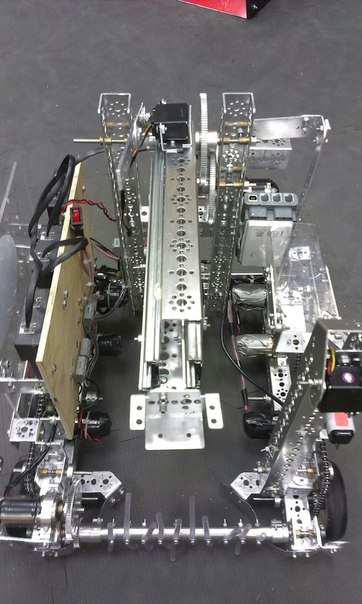
\includegraphics[scale=0.5]{days_L/Meetings/images/14}}
				\caption{New lift (lowered position)}
			\end{minipage}
			\vfill
			\begin{minipage}[h]{1\linewidth}
				\center{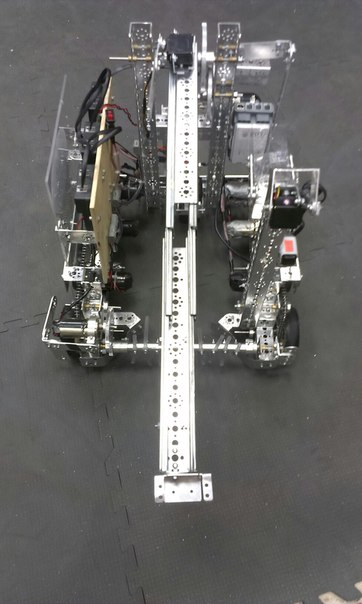
\includegraphics[scale=0.5]{days_L/Meetings/images/15}}
				\caption{Rised position}
			\end{minipage}
		\end{figure}
		
		\item It was invented idea with small wheels that rise robot when they balk the churro.
	\subsubsection{14.01.15}
		\item It was hold wires for controllers power.
	\subsubsection{16.01.15}
		\item They were mounted small wheels that provide climbing to mountain.
		\begin{figure}[H]
			\begin{minipage}[h]{1\linewidth}
				\center{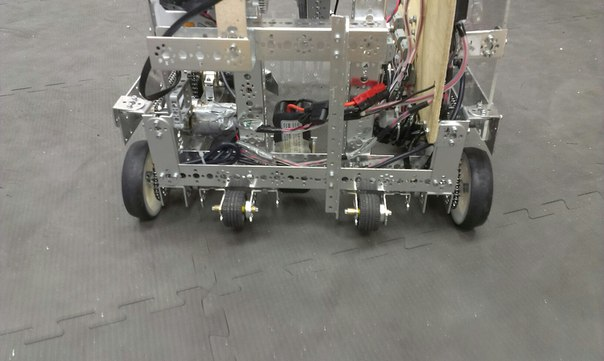
\includegraphics[scale=0.5]{days_L/Meetings/images/13}}
				\caption{Small wheels for climbing}
			\end{minipage}
		\end{figure}
		
		\item It was hold wires for motors power.
	\subsubsection{18.01.15}
		\item It was tested climbing to mountain. Robot can't climb because it rise by wheels on too smal height. So it was decided slightly lower them. After that robot was able to climb to low zone and hook by back wheels to first churro. But robot must stay at a slight angle to churro for climbing so that firstly it climb by one wheel pair then - by other. So operator that control robot's movement should train to climb to the ramp.
		
		\item In addition it was made plexiglass protection for controllers.
		\begin{figure}[H]
			\begin{minipage}[h]{1\linewidth}
				\center{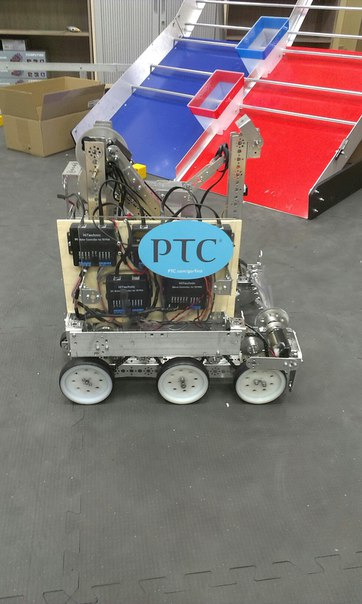
\includegraphics[scale=0.5]{days_L/Meetings/images/12}}
				\caption{Protection for controllers}
			\end{minipage}
		\end{figure}
	\subsubsection{20.01.15}	 
		\item Today we trained in climbing to mountain. During it one caterpillar torned. So we need remove them and test climbing without caterpillars.
	\subsubsection{21.01.15}
		\item Caterpillars were removed from wheels and it was tested climbing to mountain. It can move through the first churro by back and middle wheels. After that it can't move because beams on which mounted wheels touch churro. So we need to whittle down bottom part of it. 
		 	
\end{itemize}
\fillpage